\documentclass[a4paper,12pt]{article}
\usepackage[a4paper,top=1.3cm,bottom=2cm,left=1.5cm,right=1.5cm,marginparwidth=0.75cm]{geometry}
\usepackage{cmap}
\usepackage{mathtext}
\usepackage[T2A]{fontenc}
\usepackage[utf8]{inputenc}
\usepackage[english,russian]{babel}
\usepackage{siunitx}
\usepackage{enumitem}
\usepackage{placeins}

\usepackage{graphicx}

\usepackage{wrapfig}
\usepackage{tabularx}
\usepackage{multirow}

\usepackage{hyperref}
\usepackage[rgb]{xcolor}
\hypersetup{
colorlinks=true,urlcolor=blue
}
\usepackage{siunitx}
\usepackage{amsmath,amsfonts,amssymb,amsthm,mathtools}
\usepackage{icomma}
\mathtoolsset{showonlyrefs=false}
\usepackage{euscript}
\usepackage{mathrsfs}
\DeclareMathOperator{\sgn}{\mathop{sgn}}
\newcommand*{\hm}[1]{#1\nobreak\discretionary{}
{\hbox{$\mathsurround=0pt #1$}}{}}

%%% Заголовок
\newcommand\labname{Разрешающая способность микроскопа\\ (метод Аббе)}
\newcommand\labnumber{4.3.3}


\author{Макаров Лев Евгеньевич}
\title{Лабораторная работа №\labnumber

\labname
}

\date{\today}

\begin{document}

\begin{titlepage}
	\begin{center}
		{\large МОСКОВСКИЙ ФИЗИКО-ТЕХНИЧЕСКИЙ ИНСТИТУТ (НАЦИОНАЛЬНЫЙ ИССЛЕДОВАТЕЛЬСКИЙ УНИВЕРСИТЕТ)}
	\end{center}
	\begin{center}
		{\large Физтех-школа фотоники, электроники и молекулярной физики}
	\end{center}
	
	
	\vspace{4.5cm}
	{\huge
		\begin{center}
			{\bf Отчёт о выполнении лабораторной работы \labnumber}\\
			\labname
		\end{center}
	}
	\vspace{2cm}
	\begin{flushright}
		{\LARGE Автор:\\ Макаров Лев Евгеньевич \\
			\vspace{0.2cm}
			Б04-306}
	\end{flushright}
	\vspace{8cm}
	\begin{center}
		Долгопрудный 2025
	\end{center}
\end{titlepage}

\section{Введение}

\textbf{Цель работы:} 
\begin{enumerate}
	\item Определение дифракционного предела разрешения объектива микроскопа методом Аббе.
\end{enumerate}

\textbf{В работе используются:} лазер, кассета  с набором сеток разного периода, линзы, щель с микрометрическим винтом, оптический стол с набором рейтеров и крепежных винтов, экран, линейка.


\section{Теоретические сведения}

Всякая оптическая система, предназначенная для получения изображений, имеет конечный предел разрешения, т. е. ограниченную возможность раздельного наблюдения близко расположенных предметов. Принципиальной причиной, ограничивающей предел разрешения, является дифракция световых волн. Разрешающей способностью оптического прибора называют минимальное расстояние $l_{min}$ между двумя точками в пространстве предметов, которое прибор может разрешить. При визуальном наблюдении изображения в качестве критерия разрешения применяют так называемый критерий Рэлея.

Для иммерсионного микроскопа (объект находится в иммерсионной среде -- жидкости с показателем преломления n) разрешающая способность объектива при некогерентном освещении

\begin{equation*}
    l_{min}\approx\frac{0,61\lambda}{n sin A},
\end{equation*}
где $A$ — апертурный угол объектива микроскопа (см. рис. \ref{ust}), т. е. угол между оптической осью и лучом, направленным из центра объекта в край линзы.

Рассмотрим теперь когерентно освещённый объект, наблюдаемый в микроскоп. Схема образования изображения в объективе микроскопа представлена на рис. \ref{ust}. Для простоты рассмотрим случай, когда предметом является периодическая структура (дифракционная решётка), освещаемая параллельным пучком лучей. При наблюдении в микроскоп предмет располагается вблизи переднего фокуса объектива. При освещении решётки волнами, наклонными к оси, с углом наклона чуть меньшим апертуры $A$ волны нулевого порядка сфокусируются на край диафрагмы. Для получения изображения достаточно, чтобы на противоположные края сфокусировались волны 1-го порядка, т. е. угол между волнами 0 и 1 порядка должен быть равен $2A$. Минимальное разрешаемое объективом расстояние определяется условием

\begin{equation}
    l_{min} \approx\frac{\lambda}{sinA} \approx\frac{\lambda}{D/2f},
    \label{diaf}
\end{equation}
где $D$ — диаметр диафрагмы. При этом диафрагма, расположенная симметрично, пропускает нулевой и $\pm 1$ дифракционные максимумы.


В нашей работе применяется двумерная решётка -- сетка. Её можно рассматривать как две скрещенные (перпендикулярные друг к другу) решётки. Узкий пучок монохроматического света, пройдя через решётку с вертикальными штрихами, даёт совокупность максимумов, расположенных вдоль горизонтальной линии. Световой пучок, соответствующий каждому максимуму, проходя через вторую решётку, распадается на новую совокупность световых пучков, дающих максимумы вдоль вертикальной линии. Главные максимумы возникают тогда, когда одновременно выполняются условия:

\begin{equation}
    dsin\theta_x = m_x\lambda,\  \  dsin\theta_y=m_y\lambda
\end{equation}
где $m_x$ и $m_y$ — целые числа, характеризующие порядки дифракцион- ных максимумов, $\theta_x$ и $\theta_y$ — направления на главные дифракционные максимумы в горизонтальной и вертикальной плоскостях соответственно.


\textit{Разрешающей способностью оптического прибора} называют минимальное расстояние $l_{\min}$ между двумя точками в пространстве предметов, изображения которых разрешаются по методу Релея. Эту величину можно рассчитать для лупы и прочих оптических приборов.
	
\begin{figure}[h]
    \begin{center}
        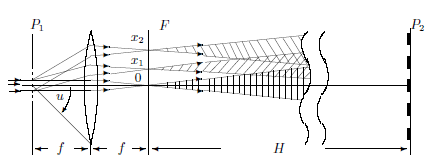
\includegraphics[width = 0.7\textwidth]{pics/433-1.png}
        \caption{Образование изображения в объективе микроскопа.}
    \label{ust}
    \end{center}
\end{figure}

Если наблюдения ведутся при внешнем освещении, то когерентные волны рассеивают различные точки предмета. Схема образования изображения представлена на рис. 1.

\section*{Подход Аббе к нахождению разрешающей способности микроскопа}
Разобьем путь лучей от предмета к изображению на 2 этапа:
\begin{enumerate}
    \item Картина, возникающая в задней фокальной плоскости $F$ --- \textit{первичное изображение}. 
    \item Первичное изображение --- источник волн $\Rightarrow$. Из этих волн возникает \textit{вторичное изображение}.
\end{enumerate}

Легко видеть, что первичное изображение представляет собой картину дифракции Фраунгофера. 

\begin{figure}[h]
    \begin{center}
        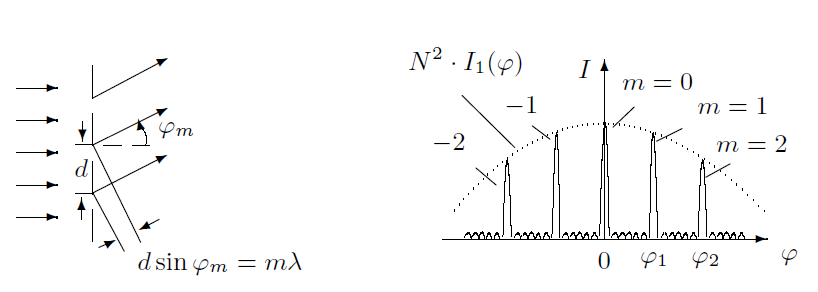
\includegraphics[width = 0.8\textwidth]{pics/433-2.png}
        \caption{Спектр амплитудной решетки}
    \end{center}
\end{figure}
При дифракции Фраунгофера на решетке периода $d$ направления $\varphi_m$ максимальной интенсивности определяются из условия 
\begin{equation}
d \sin \varphi_m = m \lambda
\end{equation}

Из рис. 2 легко видеть, что у различных максимумов разные интенсивности.
В итоге у нас излучение точечных источников на равном расстоянии, отсюда интерференция. 

При таком рассмотрении, из того, что линза конечна следует, что есть дифракционные искажения, так как проходят только те волны, для которых верно 
\begin{equation}
\varphi_m < u
\end{equation}

где $u$ --- \textit{апертурный угол} (см. рис. 1).

\begin{wrapfigure}{r}{0.35\textwidth}
    \begin{center}
        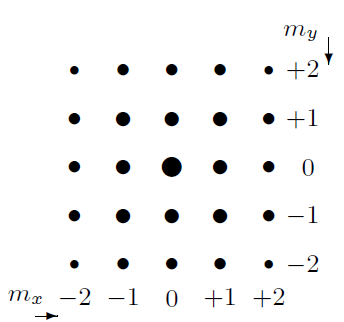
\includegraphics[width = 0.25\textwidth]{pics/433-3.png}
    \end{center}
    \caption{Дифракция Фраунгофера на двумерной решетке}\label{fraungofer}
\end{wrapfigure}

Если приоткрыть диафрагму и пустить нулевой и один из первых максимумов, то получим периодическую картинку, рассчитаем период. $x_1$ между нулевым и первыми максимумами:
\begin{equation}
x_1 \approx f \varphi_1 = f \lambda/d
\end{equation} 

Ширина интерференционных полос:
\begin{equation}
l = \lambda/\omega
\end{equation} 

где $\omega = x_1/H$ --- угол схождения интерферирующих лучей в точке наблюдения, а $H$ --- расстояние между $F$ и $P_2$. Таким образом, 
\begin{equation*}
l \approx \lambda H/x_1 = H d/f
\end{equation*}

\begin{equation*}
d' \approx \dfrac{H + f}{f} d
\end{equation*}
	
Условие разрешения решетки с периодом $d$:
\begin{equation*}
\sin u \geqslant \lambda/d \Rightarrow 
\end{equation*}

\begin{equation}
d \geqslant \dfrac{\lambda}{\sin u} \approx \dfrac{\lambda}{D/2f}
\end{equation}
Если есть не только 0 максимум, то 
\begin{equation}
d \geqslant \dfrac{\lambda}{2 \sin u}
\end{equation}

У нас решетка двумерная, поэтому мы можем записать все тоже самое в двух осях и получить картину как на рис. \ref{fraungofer}.


\section{Экспериментальная установка}

Схема модели проекционного микроскопа приведена на рис. \ref{micro}. Предметом служат сетки, расположенные в кассете. Смена сеток осуществляется поворотом внешнего кольца кассеты.

\begin{figure}[!ht]
    \centering
    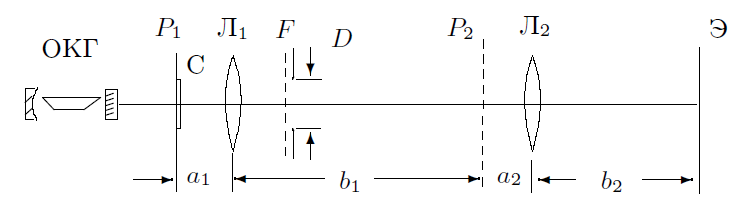
\includegraphics[width=0.9\linewidth]{pics/433-4.png}
    \caption{Схема экспериментальной установки — модель проекционного микроскопа}
    \label{micro}
\end{figure}

Излучение лазера (ОКГ) почти перпендикулярно падает на сетку С, установленную вблизи фокальной плоскости линзы Л$_1$ -- объектива микроскопа. Обычно и объектив, и окуляр микроскопа -- короткофокусные линзы (1–3 см). В нашей модели линза Л$_1$ выбирается достаточно длиннофокусной ($f \approx 10$ см), т. к. размер первичного изображения в фокальной плоскости $F$ должен быть не слишком малым, чтобы дополнительными диафрагмами можно было влиять на вторичное изображение в плоскости $P_2$. Вторичное изображение из плоскости $P_2$ проецируется на экран Э линзой Л$_2$ (короткофокусной, чтобы изображение на экране было крупнее). Во избежание микротравм глаза от излучения лазера не следует использовать эту линзу традиционным образом как окуляр микроскопа.
Изображение сетки периодически повторяется -- \textit{репродуцируется} -- в пространстве между сеткой и первой линзой, поэтому для того, чтобы среди множества репродуцированных изображений сетки можно было выделить её геометрическое изображение, на сетках изображён лисёнок, т. е. непериодический объект, изображение которого не репродуцируется.
В фокальной плоскости $F$ могут быть установлены диафрагмы — щелевая или ирисовая (отверстие с переменным диаметром) и различного рода маски (препятствия).
Как видно из соотношения \eqref{diaf}, минимально разрешимый шаг решётки или сетки определяется апертурным углом A объектива. Обычно апертура микроскопа меняется при помощи ирисовой диафрагмы на объективе (на линзе Л$_1$ такая диафрагма есть), но в наших условиях удобнее располагать щелевую диафрагму в плоскости $F$. Имея набор сеток с различными периодами $d$ и изменяя апертурный угол объектива с помощью щелевой диафрагмы, можно экспериментально проверить соотношение \eqref{diaf}.

\section{Результаты измерений и обработка данных}

\subsection*{I. Определение периода решеток по их пространственному спектру}

\begin{enumerate}
    \item Включим в сеть блок питания лазера. Следить будем за центральным лучом на его выходе.
    \item Поставим кассету с решетками перед выходным окном лазера. Пронаблюдаем на экране дифракционную картину для разных сеток. Измерим расстояние между двумя удаленными максимумами и сосчитаем число промежутков между ними. Результаты измерений запишем в таблицу \ref{table:1}.
\end{enumerate}

\begin{table}[!ht]
    \centering
    \caption{Измерение периодов решеток}
    \begin{tabular}{|l|l|l|l|l|}
        \hline
        сетка & $l$, мм & $m$ & $d$, мкм & $\sigma_d$, мкм \\ \hline
        1 & 266 & 4 & 9.92 & 0.05 \\ \hline
        2 & 265 & 10 & 24.9 & 0.1 \\ \hline
        3 & 242 & 18 & 49.0 & 0.2 \\ \hline
    \end{tabular}
    \label{table:1}
\end{table}

\begin{enumerate}[resume]
    \item Измерим расстояние от кассеты до экрана $L = 124$ см. Длина волны излучения лазера $\lambda = 532$ нм.
\end{enumerate}

\subsection*{II. Определение периодов решеток по изображению, увелиsченному с помощью модели микроскопа}

\begin{enumerate}[resume]
    \item Соберем модель проекционного микроскопа, как показано на рис. \ref{micro}.
    \item Определим расстояния $a_1, a_2, b_1, b_2$. $a_2 \approx f_2$. Поэтому измерим сразу длину тубуса $(b_1 + a_2)$. Увеличение системы найдем как:
\end{enumerate}

\begin{equation*}
    \Gamma = \frac{b_1 b_2}{a_1 a_2} = \frac{4.5 \cdot 97}{11.5 \cdot 11} \approx 3.45
\end{equation*}

Измерим периоды изображений сеток на экране и результаты измерений запишем в таблицу \ref{table:2}.

\begin{table}[!ht]
    \centering
    \caption{Измерение периодов решеток через увеличенное изображение}
    \begin{tabular}{|l|l|l|l|l|}
        \hline
        сетка & $l$, мм & $m$ & $d$, мкм & $\sigma_d$, мкм \\ \hline
        1 & 292 & 1 & 7.80 & 0.05 \\ \hline
        2 & 439 & 4 & 20.7 & 0.1 \\ \hline
        3 & 440 & 8 & 41.4 & 0.3 \\ \hline
    \end{tabular}
    \label{table:2}
\end{table}

\subsection*{III. Определение периода решёток по оценке разрешающей способности микроскопа}

\begin{enumerate}[resume]
    \item Поместим щелевую диафрагму с микрометрическим винтом в фокальную плоскость Л1. Для каждой щели определим минимальный размер $D$, при котором видно изображение решетки. Результаты измерений запишем в таблицу \ref{table:3}.
\end{enumerate}

\begin{table}[!ht]
    \centering
    \caption{Измерение $D_{\min}$ для сеток}
    \begin{tabular}{|l|l|l|}
        \hline
        сетка & $D_{\min}$, мм & $l_{\min}$, мкм  \\ \hline
        1 & $>4$ & ~  \\ \hline
        2 & $>4$ & ~  \\ \hline
        3 & 2.4 & 48  \\ \hline
    \end{tabular}
    \label{table:3}
\end{table}

\subsection*{IV. Пространственная фильтрация и мультиплицирование}

\begin{enumerate}[resume]
    \item Проведем опыт по пространственной фильтрации. Установим ширину щели так, чтобы она пропускала только максимумы нулевого порядка. Проведем измерения, когда решетка повернута вертикально, горизонтально и под углом $45^\circ$. Результаты измерений запишем в таблоицу \ref{table:4}.
\end{enumerate}

\begin{table}[!ht]
    \centering
    \caption{Измерение периодов решеток через увеличенное изображение}
    \begin{tabular}{|l|l|l|l|l|}
        \hline
        положение & $l$, мм & $m$ & $d$, мкм & $\sigma_d$, мкм \\ \hline
        вертикально & 450 & 8 & 117.28 & 0.05 \\ \hline
        горизонтально & 320 & 6 & 123.2 & 0.1 \\ \hline
        наклонная & 300 & 4 & 120.0 & 0.3 \\ \hline
    \end{tabular}
    \label{table:4}
\end{table}

\begin{enumerate}[resume]
    \item Для наблюдения мультиплицирования поменяем местами сетку и щель. Подберем ширину щели так, чтобы можно было наблюдать мультипликацию для всех сеток $D = 1$ мм.
\end{enumerate}

При уменьшении ширины картина растягивается и число мультипликаций увеличивается. При смене сеток меняется размер пропорционально периоду сетки.

\newpage
\subsection*{V. Обработка результатов}

\begin{enumerate}
    \item По измерениям спектров определим дифракционные углы и рассчитаем периоды решеток.
    \item По увеличенным изображениям рассчитаем периоды решеток еще раз. Результаты примерно совпали.
    \item По измерениям со щелью рассчитаем разрешающую способность микроскопа. Она совпала по порядку с периодом решетки.
    \item График зависимости $d = f(1/D)$ построить не вышло, так как получилось измерить только одну точку из-за недостаточной максимальной ширины решетки.
\end{enumerate}



\end{document}